\section*{Microeconomics Midterm 2016 / 17 (2)}

There are somehow two midterms for this year. This is one of the exams.

{
\subsection*{Schmidt}

\subsubsection*{Exercise 1}

Make table showing affordability \& revealed preferences. Get $w$ by Wales Law.

\begin{table}[!htp]
    \centering
    \begin{tabular}{l|c|c|c|c|l}
        $t$ & $t^{\prime}$ & $p^{t} x^{t}$ &  & $w^{t}$ & reveled preference \\
        \hline \multirow{2}{*}{0} & 1 & 96 & $>$ & 84 & - \\
        \cline { 2 - 6 } & 2 & 80 & $<$ & 84 & $x^{0}>x^{2}$ \\
        \hline \multirow{2}{*}{1} & 0 & 33 & $<$ & 36 & $x^{1}>x^{0}$ \\
        \cline { 2 - 6 } & 2 & 39 & $>$ & 36 & - \\
        \hline \multirow{2}{*}{2} & 0 & 52 & $>$ & 50 & - \\
        \cline { 2 - 6 } & 1 & 48 & $<$ & 50 & $x^{2}>x^{1}$ \\
        \hline
    \end{tabular}
\end{table}

\begin{enumerate}[label=(\alph*)]
{\item 
Violation of WARP occurs if $p^{\prime} x \leqslant w^{\prime}$ and $p x^{\prime} \leqslant w$

As we see in the table, this does not occur.

Therefore, WARP is satisfied.
}
{\item 
Looking at the last column, we find

$$
x^{0}>x^{2} \text { and } x^{1}>x^{0}
$$

Transitivity implies $x^{1}>x^{2}$. But this is violated by the last rows of the table.
}
\end{enumerate}
}
{
\subsubsection*{Exercise 2}

\begin{enumerate}[label=(\alph*)]
{\item 
Apply Roy's identity:

$$
x_{1}(p, w)=-\frac{\frac{\partial v \left(p, w\right)}{\partial p_{1}}}{\frac{\partial \left(p, w\right)}{\partial w}}=-\frac{-\frac{w}{p_{1}^{2}}}{\frac{1}{p_{1}}+\frac{1}{p_{2}}}=\frac{w}{p_{1} }\frac{1}{1+p_{1} / p_{2}}
$$
}
{\item 
(1) Invert $v(p, w)$. In equilibrium: 

$$
v(p, w)=u \quad ; \quad w=e(p, w)
$$

$$
e(p, u)=u\left[\frac{1}{p_{1}}+\frac{1}{p_{2}}\right]^{-1}
$$

(2) Apply Shepherd's Lemma:

$$
\begin{aligned}
h_{1}(p, u)=\frac{\partial e(p, u)}{\partial p_{1}} & =u(-1)\left[\frac{1}{p_{1}}+\frac{1}{p_{2}}\right]^{-2}(-1)\left(\frac{1}{p_{1}}\right)^{2} \\
& =\frac{u}{\left(1+p_{1} / p_{2}\right)^{2}}
\end{aligned}
$$
}
{\item 
$$
x_{1}\left(\lambda p_{1} \lambda w\right)=\frac{\lambda w}{\lambda p_{1}} \frac{1}{1+\frac{\lambda p_{1}}{\lambda p_{2}}}=\frac{w}{p_{1}} \frac{1}{1+p_{1} / p_{2}}=x_{1}\left(p_{1} w\right)
$$

Yes, it is.
}
{\item 
Let $f(\cdot)$ be such a monotonic transformation and apply it to $v(p, w)$. Then use Roy's identity:

$$
\begin{aligned}
& \tilde{x}_{l}(p, w)=-\frac{\frac{\partial f(v(p, w)}{\partial p_{l}}}{\frac{\partial f(v(p, w)}{\partial w}} \stackrel{*}{=}-\frac{\frac{\partial f(v(p, w))}{\partial v(p, w)}}{\frac{\partial f(v(p, w))}{\partial v(p, w)}} \frac{\frac{\partial v(p, w)}{\partial p_{i}}}{\frac{\partial v(p, w)}{\partial w}} \\
& =-\frac{\frac{\partial v\left(p_{1} w\right)}{\partial p_{1}}}{\frac{\partial v(p, w)}{\partial w}}=x_{l}(p, w)
\end{aligned}
$$

The step at * uses the chain rule to expand the expression. We see that the Walrasian demand remains the same, irrespective of the transformation.
}
\end{enumerate}
}
{
\subsubsection*{Exercise 3}

\begin{enumerate}[label=(\alph*)]
{\item 
\underline{if:}

$$
\begin{aligned}
& u(x)=\alpha-\beta \exp (-c x) \\
& u^{\prime}(x)=\beta c \cdot \exp (-c x) \\
& u^{\prime \prime}(x)=-\beta c^{2} \exp (-c x) \\
& r(x)=-\frac{u^{\prime \prime}(x)}{u^{\prime}(x)}=-\frac{-\beta c^{2} \exp (-c x)}{\beta c \exp (-c x)}=c
\end{aligned}
$$

\underline{only if:}

$$
\begin{aligned}
& c=-\frac{u^{\prime \prime}(x)}{u^{\prime}(x)}=-\frac{\partial \ln \left(u^{\prime}(x)\right)}{\partial x} \\
& \Leftrightarrow \int_{\underline{x}}^{x} \frac{\partial \ln \left(u^{\prime}(t)\right)}{\partial t} d t=\int_{\underline{x}}^{x}-c d t \\
& \Leftrightarrow \quad \ln \left(\frac{u^{\prime}(x)}{u^{\prime}(\underline{x})}\right)=-c x+c \underline{x} \\
& \Leftrightarrow \quad u^{\prime}(x)=u^{\prime}(\underline{x}) \exp (-c x+c \underline{x}) \\
& \Leftrightarrow \quad \int_{\underline{x}}^{x} u^{\prime}(y) d y=\int_{\underline{x}}^{x} u^{\prime}(\underline{x}) \exp (-c y+c \underline{x}) d y \\
& \Leftrightarrow u(x)-u(\underline{x})=u^{\prime}(\underline{x}) \exp (c \underline{x}) \frac{1}{-c}[\exp (-c x)-\exp (-c \underline{x})] \\
& \Leftrightarrow u(x)=u^{\prime}(\underline{x}) \exp (c \underline{x}) \frac{1}{-c}[\exp (-c x)-\exp (-c \underline{x})]+u(\underline{x}) \\
&=\alpha-\beta \exp (-c x)
\end{aligned}
$$
}
{\item 
Investor maximizes expected utility:

$$
\max _{a} \int u(w-a+a z) d \mp(z)
$$

Assume interior solution: obtain FOC:

$$
\int u^{\prime}(w-a+a z)(z-1) d F(z)=0
$$

Plug in $u(x)$. Use $u(x)=-\exp (-c x)$ as all positive affine transformations of $\alpha-\beta \exp (-c x)$ or allowed:

\begin{align*}
    & \int c \cdot \exp (-c(w-a+a z))(z-1) d F(z)=0 \\
    \Leftrightarrow & \frac{c \cdot \exp (-c w+c a) \int \exp (-c a z)(z-1) d F(z)=0}{\neq 0} \\
    \Leftrightarrow & \int \exp (-c a z)(z-1) d F(z)=0 \quad \tag{I}
\end{align*}

Equation (I) defines $\bar{a}$ implicitly and it is completely independent of $w$. Thus, as $w$ rises, $\bar{a}$ stays constant.
}
\end{enumerate}
}

\newpage
{
\subsection*{Gottardi}

\subsubsection*{Exercise 1}

\begin{enumerate}[label=(\alph*)]
{\item 

$$
M R S^{A}=2 \frac{x_{2}^{A}}{x_{1}^{A}} \stackrel{!}{=} M R S^{B}=2 \Leftrightarrow x_{2}^{A}=x_{1}^{A}
$$

PE allocations lie on $x_{2}^{A}=x_{1}^{A}$ until $x_{1}^{A}=6$. From there $x_{2}^{A}=6$.

\begin{figure}[!htp]
    \centering
    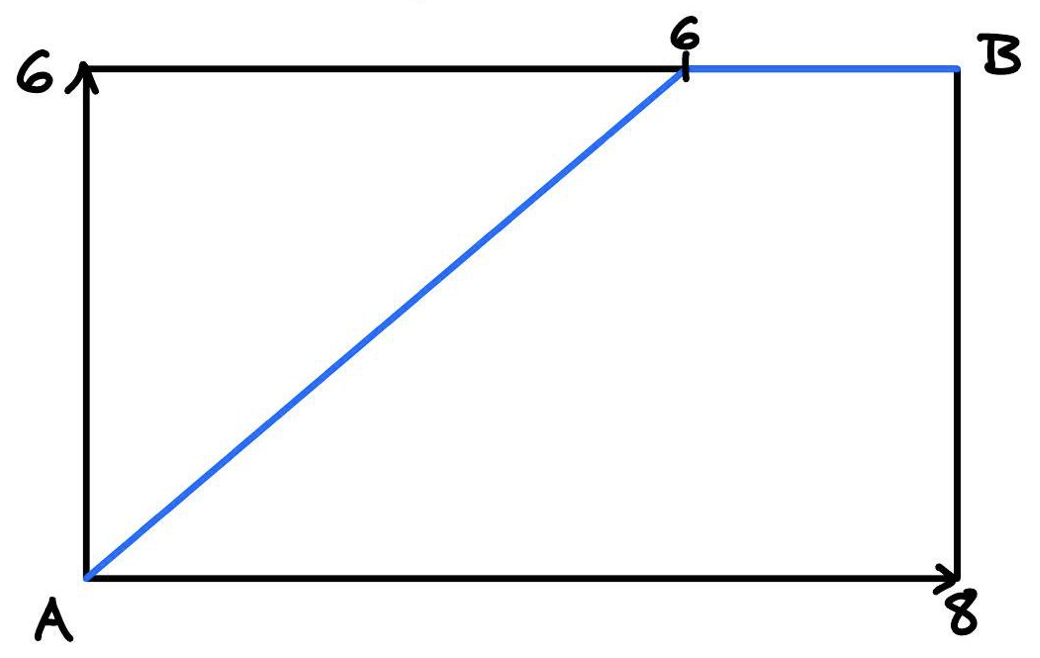
\includegraphics[width=.75\textwidth]{images/2016_17_2_1.png}
\end{figure}
}
{\item 
$$
\begin{aligned}
& U^{A}(w)=2 \ln (6)+\ln (2)=4.277 \\
& U^{B}(w)=2 \cdot 2+4=8
\end{aligned}
$$

Try new allocation (going North-East):

$$
\begin{aligned}
& u^{A}(5,3)=2 \ln (5)+\ln (3)=4.317 \\
& u^{B}(3,3)=2 \cdot 3+3=9
\end{aligned}
$$
}
{\item 
Let $p=p_{1} / p_{2}$

\underline{consumer A:}

\begin{align*}
    \max _{x_{1}^{A} x_{2}^{A}} 2 \ln \left(x_{1}^{A}\right)+\ln \left(x_{2}^{A}\right) \\
    \text{ s.t. } p x_{1}^{A}+x_{2}^{A}=p 6+2 
\end{align*}

FOCs

\begin{align*}
& \left[x_{1}^{A}\right]: \quad 2 \frac{1}{x_{1}^{\lambda}}-\lambda_{p}=0 \\
& \left[x_{2}^{A}\right]: \quad \frac{1}{x_{2}^{\lambda}}-\lambda=0 \\
& \longrightarrow x_{2}^{A}=p \frac{1}{2} x_{1}^{A} \tag{I}
\end{align*}

\underline{consumer B:}

\begin{align*}
    \max _{x_{1}^{P} x_{2}^{B}} 2 x_{1}^{B}+x_{2}^{B} \\
    \text { st. } p x_{1}^{B}+x_{2}^{B}=p_{2}+4
\end{align*}

$$
x_{1}^{B}=\left\{\begin{array}{lll}
\infty & \text { if } & p<2 \\
\mathbb{R}^{+} & \text {if } & p=2 \\
0 & \text { if } & p>2
\end{array} \quad x_{2}^{B}=\left\{\begin{array}{lll}
\infty & \text { if } & p>2 \\
\mathbb{R}^{+} & \text {if } & p=2 \\
0 & \text { if } & p<2
\end{array}\right.\right.
$$

markets: For markets to cleo (no excess demand) must have $p=2$.

Plug this into (I):

\begin{align*}
    x_{2}^{A}=x_{1}^{A} \tag{II}
\end{align*}

And this into $B C$ for $A$ :

$$
x_{1}^{A}=\frac{14}{3}=x_{2}^{A}
$$

\underline{Market Clearing:}

$$
\begin{aligned}
& x_{1}^{B}=w_{1}^{A}+w_{1}^{B}-x_{1}^{A}=8-\frac{14}{3}=\frac{10}{3} \\
& x_{2}^{B}=w_{2}^{A}+w_{2}^{B}-x_{2}^{A}=6-\frac{14}{3}=\frac{4}{3}
\end{aligned}
$$

\underline{Competitive Equilibrium:}

$$
\begin{aligned}
\left(x_{1}^{A}, x_{2}^{A}\right) & =\left(\frac{14}{3}, \frac{14}{3}\right) \\
\left(x_{1}^{B}, x_{2}^{D}\right) & =\left(\frac{10}{3}, \frac{4}{3}\right) \\
p & =2
\end{aligned}
$$

By (II) the CE is also $P E$.
}
{\item 
The price remains the same. Only the MRS of B is important for the price. If $p \neq 2$, then markets would not clear. Changing endowments does not affect the MRS of B. B's MRS is only so important because she has linear preferences, making the goods perfect substitutes for her.
}
{\item 
Equation (I) is now also valid for B. Sum over agents to see:

$$
\begin{aligned}
x_{2}^{A}+x_{2}^{B} & =p \frac{1}{2}\left(x_{1}^{A}+x_{1}^{B}\right) \\
p & =2 \frac{x_{2}^{A}+x_{2}^{B}}{x_{1}^{A}+x_{1}^{B}}
\end{aligned}
$$

By market clearing:

$$
p=2 \frac{w_{2}^{A}+w_{2}^{B}}{w_{1}^{A}+w_{1}^{B}}
$$

Therefore, the increase in $w_{1}^{B}$ decreases $P$.
}
\end{enumerate}
}
{
\subsubsection*{Exercise 2}

$$
w=(2,4)
$$

\begin{enumerate}[label=(\alph*)]
{\item 
$$
r_{1}=\left(\begin{array}{l}
2 \\
2
\end{array}\right) \quad r_{2}=\left(\begin{array}{l}
1 \\
3
\end{array}\right)
$$

Budget constraints:

\begin{align*}
a_{1} \theta_{1}+a_{2} \theta_{2}=0  \tag{III}\\
x_{1}=w_{1}+2 \theta_{1}+\theta_{2}  \tag{IV}\\
x_{2}=w_{2}+2 \theta_{1}+3 \theta_{2} \tag{V}
\end{align*}

Solve consumer problem:

$$
\begin{aligned}
& \max _{x_{1}, x_{2}} \frac{1}{2}\left(\sqrt{x_{1}}+\sqrt{x_{2}}\right) \\
& \text { sit. (III) , (IV) , (V) }
\end{aligned}
$$

Plug (IV) and (V) into objective function:

$$
\begin{aligned}
& \max _{\theta_{1} \theta_{2}} \frac{1}{2}\left(\sqrt{w_{1}+2 \theta_{1}+\theta_{2}}+\sqrt{w_{2}+2 \theta_{1}+3 \theta_{2}}\right) \\
& \text { sit. } q_{1} \theta_{1}+q_{2} \theta_{2}=0
\end{aligned}
$$

FOCs:

$$
\begin{aligned}
& \frac{1}{4}\left[\frac{2}{\sqrt{w_{1}+2 \theta_{1}+\theta_{2}}}+\frac{2}{\sqrt{w_{2}+2 \theta_{1}+3 \theta_{2}}}\right]-\lambda q_{1}=0 \\
& \frac{1}{4}\left[\frac{1}{\sqrt{w_{1}+2 \theta_{1}+\theta_{2}}}+\frac{3}{\sqrt{w_{2}+2 \theta_{1}+3 \theta_{2}}}\right]-\lambda q_{2}=0
\end{aligned}
$$

By market clearing and there only being one consumer we can set $\theta_{1}=\theta_{2}=0$:

$$
\begin{aligned}
& \frac{1}{4}\left[\frac{2}{\sqrt{w_{1}}}+\frac{2}{\sqrt{w_{2}}}\right]-\lambda q_{1}=\frac{1}{4}[\sqrt{2}+1]-\lambda q_{1}=0 \\
& \frac{1}{4}\left[\frac{1}{\sqrt{w_{1}}}+\frac{3}{\sqrt{w_{2}}}\right]-\lambda q_{2}=\frac{1}{4}\left[\frac{\sqrt{2}}{2}+\frac{3}{2}\right]-\lambda q_{2}=0 \\
& \longrightarrow \frac{q_{1}}{q_{2}}=\frac{1+\sqrt{2}}{3+\sqrt{2}} 2
\end{aligned}
$$

\underline{Competitive Equilibrium:}

The CE is a non-trade equilibrium. As preferences are convex, the CE is unique.

$$
\begin{aligned}
\left(x_{1}, x_{2}\right) & =(2,4) \\
\left(\theta_{1}, \theta_{2}\right) & =(0,0) \\
\frac{q_{1}}{q_{2}} & =2 \frac{1+\sqrt{2}}{3+\sqrt{2}}
\end{aligned}
$$
}
{\item 
Note: in reality, we only know $q_{1} / q_{2}$. Thus we can only compare the expected rates of return but not calculate their absolute values:

$$
\begin{aligned}
& \frac{a_{1}}{q_{2}}=2 \frac{1+\sqrt{2}}{3+\sqrt{2}}>1=\frac{\mathbb{E}\left(r_{1}\right)}{\mathbb{E}\left(r_{2}\right)} \\
\Rightarrow & \frac{\mathbb{E}\left(r_{1}\right)}{q_{1}}<\frac{\mathbb{E}\left(r_{2}\right)}{q_{2}}
\end{aligned}
$$

Asset two has the higher rate of expected return. We already know that this is only due to a higher relative price of asset 1. Asset 1 has to be more expensive, otherwise the consumer would buy it to insure herself against poorer state 1 as she is strictly risk-averse. She is alone in the market \& thus the excess demand for asset 1 increases its relative price.
}
{\item 
No. The market was already complete. The new
asset is a linear combination of the others and it introduces no new choice option for the consumer.
}
\end{enumerate}
}